%%%%%%%%%%%%%%%%%%%%%%%%%%%%%%%%%%%%%%%%%%%%%%%%%%%%%%%%%%%%%%%%%%%%%%
% How to use writeLaTeX: 
%
% You edit the source code here on the left, and the preview on the
% right shows you the result within a few seconds.
%
% Bookmark this page and share the URL with your co-authors. They can
% edit at the same time!
%
% You can upload figures, bibliographies, custom classes and
% styles using the files menu.
%
%%%%%%%%%%%%%%%%%%%%%%%%%%%%%%%%%%%%%%%%%%%%%%%%%%%%%%%%%%%%%%%%%%%%%%

\documentclass[12pt]{article}

\usepackage{sbc-template}

\usepackage{graphicx,url}

%\usepackage[brazil]{babel}   
\usepackage[utf8]{inputenc}  
\usepackage{amsmath,amssymb}
\usepackage{float}
\usepackage{tikz}
\usepackage{listings}
\lstdefinelanguage{HTML}{
  keywords={class, export, boolean, throw, implements, import, this, const, v-model, require}
  keywordstyle=\color{blue}\bfseries,
  ndkeywords={},
  ndkeywordstyle=\color{darkgray}\bfseries,
  identifierstyle=\color{darkgray},
  sensitive=false,
  comment=[l]{//},
  morecomment=[s]{/*}{*/},
  stringstyle=\color{teal}\ttfamily,
  commentstyle=\color{purple}\ttfamily,
  morestring=[b]',
  morestring=[b]",
  morestring=[b]`,
  basicstyle=\small
}

     
\sloppy

\title{Intuitive Management Interface for Graph Database}

\author{Filipe S. P. Prates\inst{1} }


\address{Universidade Federal do Rio de Janeiro
  (UFRJ)\\
    Caixa Postal 68511 CEP: 21941-972  Rio de Janeiro - RJ - Brasil
  \email{filipeprates@poli.ufrj.br}
}

\begin{document} 

\maketitle

\begin{abstract}
This article describes an intuitive interface for management of graph data, allowing for easy navigation and arbitrary manipulation of the nodes and edges. As an example, it describes an implementation using a Neo4j database that is managed through a GraphQL API and a Vue.js web interface. 

\end{abstract}

\begin{resumo}   Este artigo descreve uma interface intuitiva para gerenciamento de dados armazenados em grafos, permitindo exploração e manipulação arbitrária dos nós e relações. Como exemplo é descrito uma implementação utilizando bancos de dados Neo4j, através de uma API em Graphql, e uma interface desenvolvida em Vue.js.

\end{resumo}


\section{Informações Gerais}

As ferramentas disponíveis de gerenciamento de dados armazenados em bancos de dados baseados em grafos, em especial o banco de dado Neo4j Database \cite{Neo4j}, se limitam à interações diretas por DCL (Data Control Language / Linguagem de Controle de Dados) \cite{Cypher} e provêm ao usuário resultados como visualizações gráficas de subgrafos e tabelas. Quando tais dados são gerenciados por usuários sem conhecimento prévio de seu schema, os resultados e visualizações podem ser de difícil compreensão, além de existir o risco de alterações equivocadas de grande alcance nos dados.

Neste contexto, surgiu a demanda da criação de uma interface para que usuários não técnicos conseguissem visualizar e interagir com os dados armazenados em um banco de dados em grafo.

\section{Interface em ``Pefis e Listas''}

A interface desenvolvida, em ``Pefis e Listas'', recebe o schema do banco de dados que está associada (através da requisição \textit{InformationSchema}), e através de um template de página de Perfil e de uma página de lista de nós, permite-se a criação e edição arbitrária dos nós e seus relacionamentos.

Cada nó do grafo possui então uma página de perfil, que mostra e permite edição de suas propriedades e relações. Além destas, cada \textit{rótulo} \cite{Neo4jLabels} de nó presente no banco de dados possui uma página de lista/pesquisa, onde podemos buscar e acessar as páginas de perfil de nós pertencentes ao rótulo referente.

A vantagem dessa modelagem é que conseguimos aproveitar o fato de que toda página de perfil (e de lista) segue a mesma lógica, então o código referente à sua implementação pode ser reutilizado. Ná prática, a aplicação consiste em apenas uma página de perfil e uma página de lista (além da página de login/autenticação), que são populadas dado o contexo, e ações que são comunicadas através de requisições em GraphQL genéricas, que recebem os \textit{rótulos} como argumento, permitindo assim uma mesma ação ser utilizada em diferentes contextos. Desta maneira, o tamanho do código da aplicação é minimizado, facilitando sua manutenção.

\begin{figure}[ht]
\centering
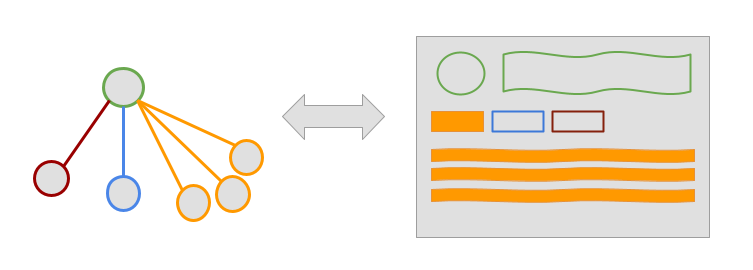
\includegraphics[width=1\textwidth]{isom.png}
\caption{Abstração de um \textbf{nó dono} (verde) está relacionado à \textbf{um nó de \textit{rótulo} X} (vermelho), \textbf{um de \textit{rótulo} Y} (azul), e possui relação com \textbf{três nós de \textit{rótulos} Z} (amarelos) no grafo armazenado no banco de dados.}
\label{fig:isom}
\end{figure}

\subsection{Página de Perfil do Nó}

A página de perfil do nó consiste nas propriedades do nó na parte superior da tela, além de, na parte inferior, uma série de abas, uma para cada diferente \textit{rótulo} de relação que o nó pode possuir.

Dentro de cada aba da página de perfil temos uma lista de elementos que representam os vizinhos do nó através de relações que contém o \textit{rótulo} identificador da aba. O usuário tem acesso á selecionar elementos e, dependendo de suas permissões, ações como Adição, Criação, Edição, Deleção, Remoção da relação, e qualquer outra que seja relevante ao \textit{rótulo} do nó, gerada através de templates em GraphQL que recebem o \textit{rótulo} da aba e do nó dono do perfil como argumentos \cite{GraphQL}, além dos identificadores dos elementos da lista que são selecionados.

Tal lista de elementos/vizinhos também possuem hiperlinks para as páginas de perfis destes nós vizinhos. Desta maneira conseguimos caminhar pelo grafo através das relações, sendo cada passo atráves dos perfis dos nós, tendo acesso à ações como edição, criação e deleção deles, além de criação/remoção de relações entre nós existentes.

\subsection{Página de Lista de Nós}

Porém é possível que o grafo armazenado no banco de dados não seja conexo, ou então que o nó que deseja gerenciar está à muitos passos de distância do nó da página de perfil atual, por um caminho não-óbvio, ou então precisamos começar a navegar pelo grafo a partir de algum nó inicial, nesses momentos é útil ao usuário uma das páginas de ``Lista'', com suas ferramentas de pesquisa.

Nestas são listados todos os nós de um certo \textit{rótulo}, de forma paginada, com hiperlinks para suas respectivas páginas de perfil. Possuem também funcionalidades de busca e filtragem genéricas, através de GraphQLs que recebem o \textit{rótulo} da lista como argumento, além de acesso à ações diretas nos elementos listados.

\begin{figure}[ht]
\centering
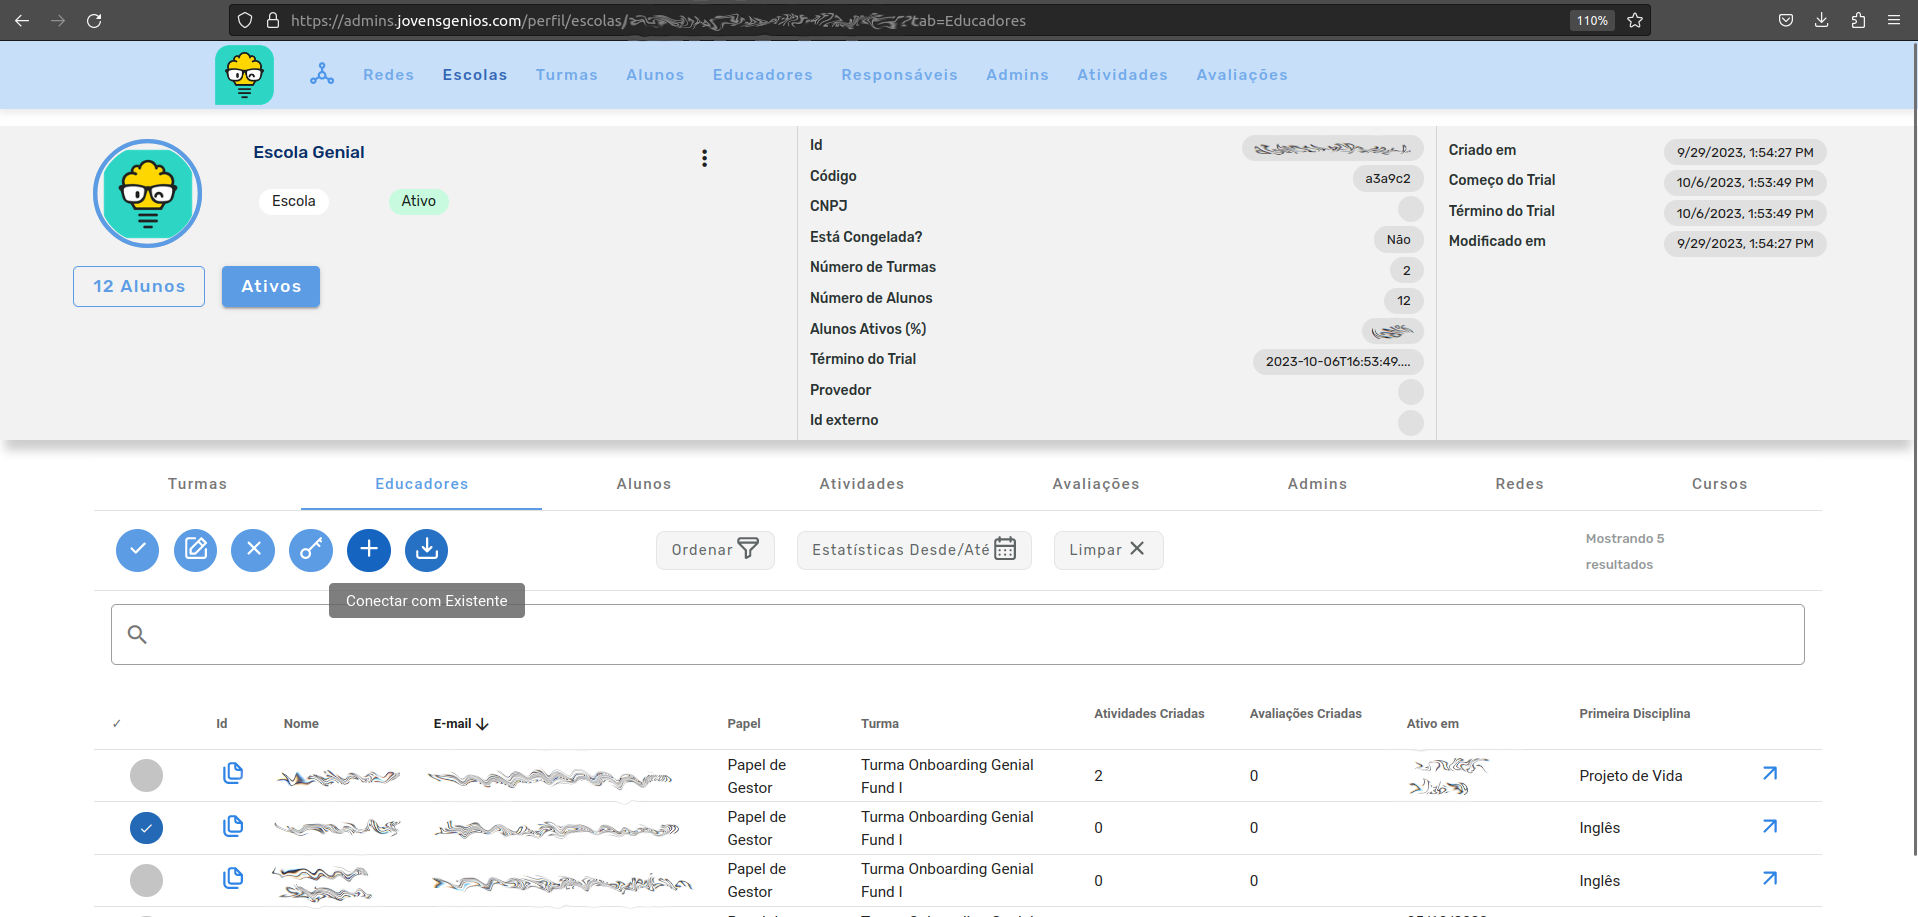
\includegraphics[width=1\textwidth]{profile-example.png}
\caption{Página de Perfil de um nó no banco de dados Neo4j que representa uma escola. Note as propriedades do nó na parte superior da tela, separadas dependendo se são de DateTime ou não, além das diferentes abas, uma para cada \textit{rótulo} de relação com vizinhos que o nó possui, estando a aba do \textit{rótulo} ``Educadores'' selecionada. Resultante desta seleção, uma lista com os vizinhos do nó escola que são nós de educadores aparece na parte inferior da tela, permitindo seleção de elementos, e ações em azul no cabeçalho da lista. Inclui seleção/deseleção de todos os nós, edição do(s) nó(s) selecionados, além de remoção e criação de relações, e outras ações.}
\label{fig:profile-example}
\end{figure}

\section{Formulário de Edição/Criação reutilizável}

Dentro do componente do formulário reutilizável, um objeto de nome \textit{properties} é criado, e vai popular o formulário conforme o \textit{rótulo} demanda, e com as informações já existentes no nó caso esteja em modo de edição.

Com as informações resultantes da requisição de introspeção, é filtrado quais as propriedades que são editáveis, e então são separadas dependendo de seu tipo. Para cada tipo de propriedade do nó, renderizamos um componente de interação específico dele no formulário. Temos assim uma série de caixas de texto, ou componentes de seleção de data, ou seletores booleanos, ou até seletores com valores fixos (enums), informados pela própra requisição de introspeção ao abrir o formulário de edição/criação deste \textit{rótulo} pela primeira vez.

Abaixo, um exemplo de renderização de diferentes componentes do formulário, dependendo de seu tipo, tal agrupamento, que define a variável \textit{properties} no exemplo, acontece ao formulário ser acessado na camada de controle de estados.
\begin{lstlisting}[language=HTML]
<form>
    <row
      v-for="(propInfo, propName) in properties.strings"
      :key="i"
    >
     <col full>
      <v-text-field
        v-model="propInfo.value"
        :label="`propName"
        :disabled="propInfo.disableEdit"
        outlined
      />
     </col>
    </row>
    <row full
      v-for="(propInfo, propName) in properties.dateTimes"
      :key="j"
    >
     <col full>
      <date-time-picker
        :datetime="propInfo.value"
        :label="`propName"
        />
      </col>
    </row>
...

\end{lstlisting}

\begin{figure}[ht]
\centering
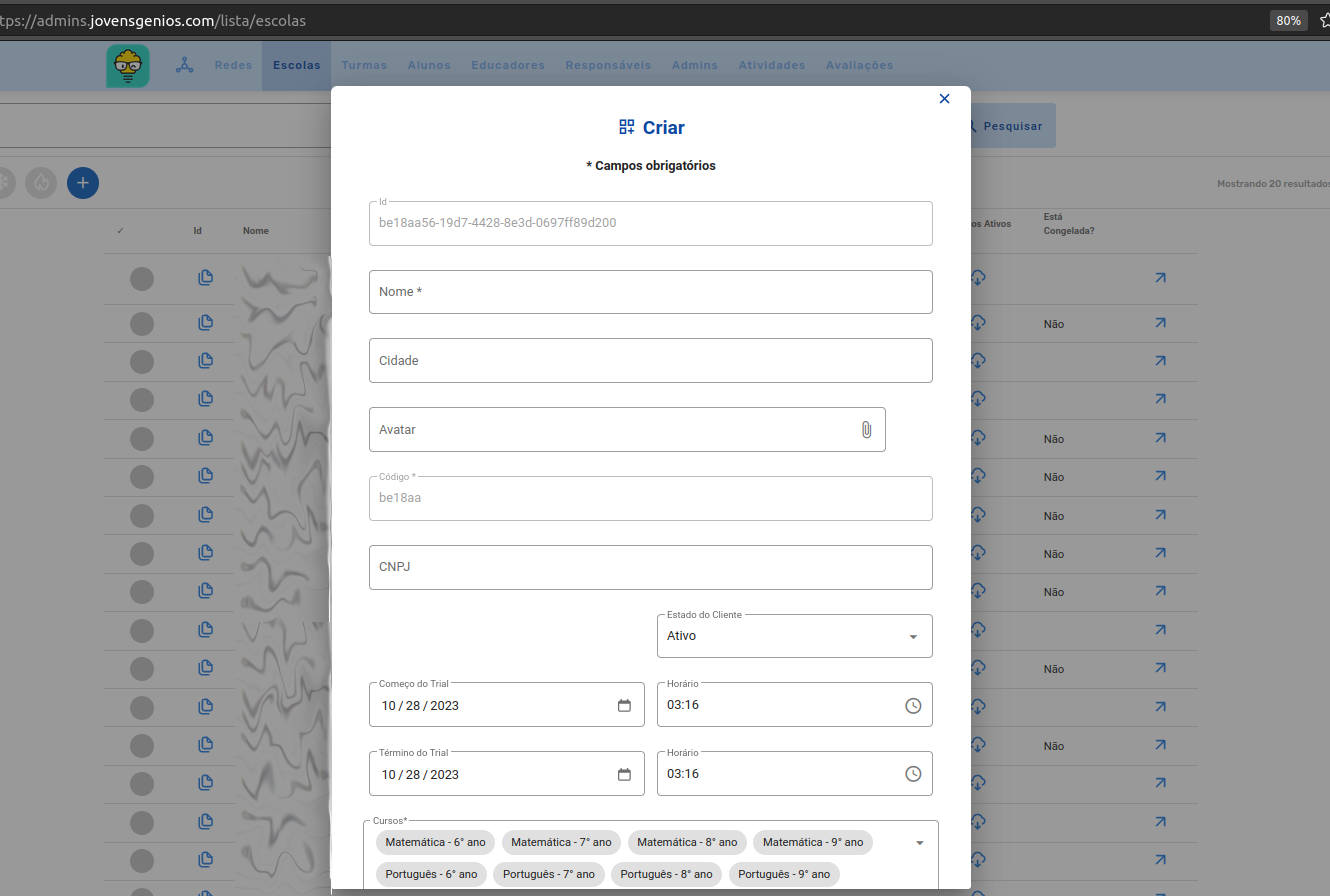
\includegraphics[width=0.8\textwidth]{reusable-form.png}
\caption{Formulário de Criação de Nó de \textit{rótulo} ``Escola'', na página de Lista de ``Escolas''. Note o componente de edição de Id disabilitado, campos de edição de string, edição de propriedades de imagens, seletor dentre possibilidades fixas, seletor de datas e seletores customizados, específicos para a criação deste \textit{rótulo} (no caso, um seletor para ao criar a escola, automaticamente conectá-la aos nós de \textit{rótulo} ``Curso'' que ela tem acesso).}
\label{fig:reusable-form}
\end{figure}

Para finalizar a interface, existe uma camada superior de controle de estado, que gerencia os formulários e ações, e popula os templates de páginas atráves das informações recebidas da \textit{InformationSchema}, a requisição de introspeção do banco de dados da biblioteca neo4j-graphql \cite{Neo4jGraphQL}.

\section{Resultados}
A abstração do grafo em ``Perfis e Listas'' se mostrou uma maneira intuitiva de navegar e interagir com os dados, sendo utilizado diariamente desde 2020 por múltiplos usuários de diversas áreas de uma empresa de tecnologia aplicada à educação para gerenciar dados armazenados em uma banco de dados Neo4j.

\section{Conclusões}
É necessária uma ferramenta para interagir com dados de maneira intuitiva e simples, possibiliando assim diversos usuários não-técnicos a gerenciarem um mesmo grafo armazenado.

A interface em ``Perfil e Listas'' simplifica a interação com um banco de dados em grafos, utilizando interfaces e navegações similiar à redes sociais, as quais os usuários já estão familizarizados.

A possibilidade de realizar uma mesma ação de manipulação de aresta através da página de perfil do nó ou da página de perfil de seu vizinho provê facilidade e rapidez na sua realização. Podendo o usuário escolher qual caminho até a ação de manipulação é mais conveniente no momento.

\bibliographystyle{sbc}
\bibliography{sbc-template}

\end{document}
